\documentclass[a4paper,12pt]{article}
% Define paper size, seperate titlepage, 12 pt. font, document class
%--------------------------------------------------------------------------------------------------
% Begin Preamble
%--------------------------------------------------------------------------------------------------
\usepackage{amsmath}
\usepackage{amssymb}
\usepackage{here}
\usepackage{graphicx}
\usepackage{epstopdf}
\usepackage{framed}
\usepackage{stmaryrd}
\usepackage{amsthm}
\usepackage{multicol}
\usepackage{manfnt}
\usepackage{fancybox}
\usepackage{pdflscape}
\usepackage{epsfig}
\usepackage{multirow}
\usepackage{color}
\usepackage{booktabs}
\usepackage{natbib}
\usepackage{lettrine}
\usepackage{appendix}
\usepackage{ifthen}
\usepackage[affil-it]{authblk}
\usepackage[utf8]{inputenc}
\usepackage[T1]{fontenc}
\usepackage{kpfonts}
\usepackage[doublespacing]{setspace}
\usepackage{csquotes}
\usepackage{subcaption}
%\usepackage{booktabs}
%\usepackage{threeparttable}
% Load Standard Packages
\usepackage{tabularx}
\newcolumntype{Y}{>{\centering\arraybackslash}X}
%Graphs and Tables to the end of the paper
\usepackage{endfloat}

%--------------------------------------------------------------------------------------------------
\usepackage{setspace}
	\onehalfspacing
% Set spacing to 1.5
%\numberwithin{figure}{section}
%\numberwithin{table}{section}
%  Number within Sections

\definecolor{deepred}{rgb}{0.803922,0,0}
%--------------------------------------------------------------------------------------------------
\usepackage{fancyhdr}
	\pagestyle{fancy}
	\headheight 35pt
	\fancyhf{}
	\rhead{}
	\chead{}
	\lhead{}
	\lhead{}
	\rfoot{\thepage}
	\cfoot{}
	\lfoot{}
	\renewcommand{\headrulewidth}{0.0pt}
	\renewcommand{\footrulewidth}{0.0pt}
% Define header and footnote styles
%--------------------------------------------------------------------------------------------------
%\usepackage[small,bf]{caption}
%\setlength{\captionmargin}{20pt}
% Makes the captions of figures/tables look nicely
%--------------------------------------------------------------------------------------------------
\usepackage[flushleft]{threeparttable}
\usepackage{ifxetex}
\usepackage[dvipsnames]{xcolor}
\ifxetex{%
  \usepackage{fontspec}
  \setmainfont{Linux Libertine O} % or any font on your system
  \newfontfamily\quotefont[Ligatures=TeX]{Linux Libertine O} % or any font on your system
\else
  \usepackage[utf8]{inputenc}
  \usepackage[T1]{fontenc}
  \usepackage{kpfonts} % or any other font package (or none)
  \newcommand*\quotefont{\fontfamily{fxl}} % selects Libertine for quote font
\fi
\usepackage{tikz}
\usepackage{framed}
% Make commands for the quotes
\newcommand*{\openquote}{\tikz[remember picture,overlay,xshift=-15pt,yshift=-10pt]
     \node (OQ) {\quotefont\fontsize{60}{60}\selectfont``};\kern0pt}
\newcommand*{\closequote}{\tikz[remember picture,overlay,xshift=15pt,yshift=10pt]
     \node (CQ) {\quotefont\fontsize{60}{60}\selectfont''};}
% select a colour for the shading
\definecolor{shadecolor}{named}{White}
% wrap everything in its own environment
\newenvironment{shadequote}%
{\begin{snugshade}\begin{quote}\openquote}
{\hfill\closequote\end{quote}\end{snugshade}}
%--------------------------------------------------------------------------------------------------
\usepackage[margin=2.3cm,includeheadfoot=false,twoside=false,bindingoffset=0.0cm,showframe=false]{geometry}
%\fancyhfoffset[E,O]{0pt}
% Add nicer enumbering of formulars
%--------------------------------------------------------------------------------------------------
\newcommand{\ws}{$^{\,\star}$}
\newcommand{\ms}{$^{\,\star \star}$}
\newcommand{\hs}{$^{\,\star \star \star}$}
\newcommand{\sym}[1]{\rlap{#1}}
% End Preamble
%--------------------------------------------------------------------------------------------------
\title{The political economy of EU asylum policies}
\date{June 2017}
\author[,1]{Martina Burmann\thanks{burmann@ifo.de}}
\author[,1]{Marcus Drometer\thanks{drometer@ifo.de}}
\author[,2]{Romuald M\'eango\thanks{meango@mea.mpisoc.mpg.de}}
\affil[1]{ifo Institute for Economic Research, Munich}
\affil[2]{Munich Center for the Economics of Aging (MEA)}
\renewcommand\Authands{ and }
%--------------------------------------------------------------------------------------------------
\begin{document}
%--------------------------------------------------------------------------------------------------
      \maketitle
%--------------------------------------------------------------------------------------------------
\begin{abstract}
\singlespacing
\noindent 
Asylum policies are partly determined by factors of political economy. However, there is little evidence on the precise linkages between political factors and asylum policies. We shed light on this issue by examining the impact of elections and parties on both applications for asylum as well as asylum recognition rates. Our evidence is based on a large bilateral panel data set comprising 11 European destination countries and their 38 most relevant origin countries during the time period 2009 to 2016. Our findings suggest that the number of first-time asylum applicants per capita are in general  lower under right-wing parties and higher under left-wing-parties. Interestingly, the number of asylum applicants under right- and left-wing parties converges before elections and differs thereafter. In contrast with the asylum seeker admission policies, the asylum decision process does not seem to be driven by electoral concerns. 
\bigskip

\textbf{Keywords}: Electoral cycles, migration policies.

\textbf{JEL}: H11, D72, F22

\bigskip
\end{abstract}
%\addtolength{\baselineskip}{.25\baselineskip}
\setcounter{page}{0} \renewcommand{\thepage}{}
\pagebreak\pagenumbering{arabic}\pagebreak

%%--------------------------------------------------------------------------------------------------
\section{Extended Abstract}\label{extended_abstract}
Since March 2016, the European Union has signed an agreement with Turkey to close off the migration route across the Aegean, one of the most popular routes for asylum-seekers from Asia. This has been done despite protests from many human rights groups that think such an agreement violates the international Convention on Refugees. In a tribune entitled ``Keep them away'', \textit{\cite{Economist2017}} describes policies intended by many EU countries as policies ``where asylum-seekers would need to apply from abroad rather than coming to Europe.'' This tension between the provision of asylum for rightfully entitled individuals and groups, and the pursuit of other political and economic goals has been acknowledged by the economic literature that compares the provision of asylum as a public good, where costs are privately assumed by the host countries \citep{moraga2014}. With this background in mind, \cite{dustmann2016} note that ``the  different  exposures  to  refugee  inflows and  the  lack  of  any  effective  European-level  mechanism  to  `spread  the  burden'  of  hosting  refugee  populations,  led  many  countries  to  implement  procedures  aimed  at  reducing  inflows  into  their  territories.''

Despite the recognition that asylum policies are partly determined by political economy factors in the destination country, there is little empirical evidence on the precise linkages between those political factors and asylum policies. We shed light on this issue by examining the impact of elections and parties on both applications for asylum as well as asylum recognition rates. 

Our evidence is based on a large bilateral panel data set from Eurostat comprising 19 European destination countries and their 40 most relevant origin countries during the time period 2008 to 2016. The dataset reports monthly origin-specific first-time asylum applications, quarterly aggregate outcomes of claims, and type of status obtained (full refugee status or some form of temporary protection\footnote{In this paper we define temporary protection to be any form of international protection other than full Geneva Convention refugee status, including temporary protection, subsidiary protection and protection on humanitarian grounds. }). Following \cite{hatton2016}, we drop country pairs with few applications (less than 100 first time applications during the time period under study), which leaves us with 464 out of 760 possible origin destination combinations. We combine this dataset with the ParlGov dataset that comprises information on European national elections (date and outcomes) and party positions \citep{parlgov2016}. We derive the position of the government on a left-right scale by weighting the left-right position of the parties in government  against the ratio of the parties' seats to the cabinet's total seats in parliament.  Next, we divide the sample of all governments into terciles  to form three cabinet groups: left, center and right-wing.

%Our results establish empirically that asylum policies are affected by the electoral cycle and the identity of incumbent parties. More precisely, we establish three main results:

%(i) before an election, the inflow of refugees is very similar across all types of cabinets (left, center or right-wing) ; 
% @Marcus: Should we use Party, government, parliament... ???

 %(ii)  in the quarters following an election, the inflow of refugees diverges substantially, with significantly less asylum applicants under a right-wing cabinet; 
 
 %(iii) in contrast with the asylum-seeker admission policies, the asylum decision process does not seem to be affected by an election.
In our main specification we estimate the following fixed-effect regression:
\begin{equation}
logApp_{ijq} =\alpha_1 \mathbf{O_{iq}} + \alpha_2 \mathbf{D_{jq}} + \alpha_3  \mathbf{C_{jq}} + \alpha_4\mathbf{Q_{j.}} + \alpha_5  [\mathbf{Q_{j.}} *  \mathbf{C_{jq}}] + \tau_q + \sigma_{ij} +  \varepsilon_{ijt},
\end{equation}where the dependent variable is the log of the number of first-time asylum applications per capita from citizens of origin country i in destination country j in quarter q.\footnote{In our paper we use the number of first time applications per capita in the destination country. \cite{hatton2016}, in contrast, uses the number of first time asylum applications per capita in the origin country. We also tried specifications with the dependent variables as \cite{hatton2016} uses it and our results do not change.} To derive this equation, we follow \cite{hatton2016}'s specification, and add to the origin and destination specific explanatory variables $\mathbf{O_{iq}}$ and $\mathbf{D_{jq}}$ , as a set of dummies for before, during and after the election ($\mathbf{Q_j.} := Q_{j,bef}, Q_{j,el}, Q_{j,aft}$) or for different quarters before and after an election in a quarter $t=0$, in destination country $j$ ($\mathbf{Q_j.} =\{Q_{jt}, t = -6, \ldots, +6\}$).  Additionally,  we include dummies for the ruling cabinet's position on a left-right scale $\mathbf{C_{jq}}$ (omitted category center)  and  interact the period-indicators $\mathbf{Q_j.}$ with the cabinet position indicators $\mathbf{C_{jq}}$.  Following \cite{hatton2016}, we include Political Terror Scale, Freedom House Index of Civic Liberties, Freedom House Index of  Political Rights, number of battle deaths and log real GDP per capita in the vector of time variant origin specific variables $\mathbf{O_{iq}}$.\footnote{All origin specific variables vary on the year level and are taken from the following sources: political terror scale from \cite{PTS2016};  Freedom House Index of Civic Liberties and Political Rights from \cite{FHI2017};  number of battle death  from the Uppsala Conflict Data Program \citep{Uppsala2017}  and real GDP per capita from the Penn World Table \citep{PWT2015}.} The vector of time variant destination variables $\mathbf{D_{jq}}$ comprises of the quarterly log real GDP per capita and the quarterly unemployment rate at destination.\footnote{Data on real GDP per capita and unemployment at the destination countries are from Eurostat.} Our main specification as described in equation (1), moreover, includes quarter-year dummies $\tau_q$ and destination-origin fixed effects $\sigma_{ij}$. In all regressions standard errors are clustered by origin country.

\begin{table}\centering
	\footnotesize
\def\sym#1{\ifmmode^{#1}\else\(^{#1}\)\fi}
\caption{Determinants of log(First time asylum applications per capita)}
\begin{tabular}{l*{6}{c}}
	\hline\hline
	&\multicolumn{1}{c}{(1)}         &\multicolumn{1}{c}{(2)}         &\multicolumn{1}{c}{(3)}         &\multicolumn{1}{c}{(4)}         &\multicolumn{1}{c}{(5)}         &\multicolumn{1}{c}{(6)}         \\
	\hline
	&\\
	Political Terror Scale                  &     0.367\sym{**} &     0.371\sym{**} &                   &     0.362\sym{**} &     0.366\sym{**} &                   \\
	&   (0.105)         &   (0.106)         &                   &   (0.105)         &   (0.106)         &                   \\
	[0.3em]
	Civic Liberty (FHI)                     &    -0.161         &    -0.173         &                   &    -0.156         &    -0.167         &                   \\
	&   (0.112)         &   (0.112)         &                   &   (0.113)         &   (0.113)         &                   \\
	[0.3em]
	Political Rights (FHI)                  &   -0.0141         &  -0.00340         &                   &   -0.0158         &  -0.00509         &                   \\
	&  (0.0767)         &  (0.0742)         &                   &  (0.0763)         &  (0.0739)         &                   \\
	[0.3em]
	Battle deaths (000s)                     &    0.0260\sym{***}&    0.0260\sym{***}&                   &    0.0259\sym{***}&    0.0259\sym{***}&                   \\
	& (0.00306)         & (0.00310)         &                   & (0.00307)         & (0.00312)         &                   \\
	[0.3em]
	log origin country real GDP per capita  &    -0.510\sym{***}&    -0.497\sym{***}&                   &    -0.513\sym{***}&    -0.500\sym{***}&                   \\
	&   (0.142)         &   (0.138)         &                   &   (0.144)         &   (0.140)         &                   \\
	[0.3em]
	log migrant stock in 2000/1             &     0.242\sym{***}&                   &     0.243\sym{***}&     0.242\sym{***}&                   &     0.243\sym{***}\\
	&  (0.0299)         &                   &  (0.0297)         &  (0.0299)         &                   &  (0.0297)         \\
	[0.3em]
	log distance from origin to destination &   -0.0515         &                   &   -0.0415         &   -0.0512         &                   &   -0.0414         \\
	&   (0.340)         &                   &   (0.342)         &   (0.341)         &                   &   (0.342)         \\
	[0.3em]
	log destination country real GDP per capita&    -1.512\sym{**} &    -1.531\sym{**} &    -1.713\sym{**} &    -1.768\sym{**} &    -1.784\sym{**} &    -1.974\sym{***}\\
	&   (0.533)         &   (0.531)         &   (0.507)         &   (0.532)         &   (0.530)         &   (0.508)         \\
	[0.3em]
	Unemployment rate at destination        &    -0.122\sym{***}&    -0.122\sym{***}&    -0.117\sym{***}&    -0.122\sym{***}&    -0.123\sym{***}&    -0.118\sym{***}\\
	&  (0.0157)         &  (0.0157)         &  (0.0155)         &  (0.0162)         &  (0.0162)         &  (0.0159)         \\
	[0.3em]
	Weighted cabinet position left          &    0.0922         &    0.0836         &    0.0885         &     0.203\sym{*}  &     0.191\sym{*}  &     0.187\sym{*}  \\
	&  (0.0488)         &  (0.0499)         &  (0.0504)         &  (0.0810)         &  (0.0837)         &  (0.0825)         \\
	[0.3em]
	Weighted cabinet position right         &    -0.439\sym{***}&    -0.444\sym{***}&    -0.432\sym{***}&    -0.704\sym{***}&    -0.708\sym{***}&    -0.713\sym{***}\\
	&  (0.0559)         &  (0.0566)         &  (0.0557)         &  (0.0767)         &  (0.0777)         &  (0.0722)         \\
	[0.3em]
	time period before the election         &    0.0876\sym{*}  &    0.0882\sym{*}  &    0.0651         &   -0.0417         &   -0.0405         &   -0.0727         \\
	&  (0.0415)         &  (0.0412)         &  (0.0408)         &  (0.0638)         &  (0.0635)         &  (0.0628)         \\
	[0.3em]
	quarter of the election                 &     0.105\sym{*}  &     0.100\sym{*}  &    0.0962         &   -0.0154         &   -0.0253         &   -0.0263         \\
	&  (0.0485)         &  (0.0492)         &  (0.0492)         &  (0.0708)         &  (0.0729)         &  (0.0706)         \\
	[0.3em]
	time period after the election          &    0.0916\sym{*}  &    0.0918\sym{*}  &    0.0761         &    0.0349         &    0.0336         &   -0.0142         \\
	&  (0.0401)         &  (0.0400)         &  (0.0391)         &  (0.0711)         &  (0.0714)         &  (0.0682)         \\
	[0.3em]
	cabinet position left * before the election&                   &                   &                   &    -0.243\sym{**} &    -0.238\sym{**} &    -0.236\sym{**} \\
	&                   &                   &                   &  (0.0816)         &  (0.0823)         &  (0.0806)         \\
	[0.3em]
	cabinet position left * election quarter&                   &                   &                   &    -0.364\sym{**} &    -0.350\sym{**} &    -0.373\sym{**} \\
	&                   &                   &                   &   (0.122)         &   (0.125)         &   (0.118)         \\
	[0.3em]
	cabinet position left * after the election&                   &                   &                   &    -0.127         &    -0.121         &   -0.0855         \\
	&                   &                   &                   &  (0.0805)         &  (0.0821)         &  (0.0805)         \\
	[0.3em]
	cabinet position right * before the election&                   &                   &                   &     0.614\sym{***}&     0.607\sym{***}&     0.631\sym{***}\\
	&                   &                   &                   &  (0.0652)         &  (0.0640)         &  (0.0610)         \\
	[0.3em]
	cabinet position right * election quarter&                   &                   &                   &     0.665\sym{***}&     0.674\sym{***}&     0.652\sym{***}\\
	&                   &                   &                   &  (0.0879)         &  (0.0883)         &  (0.0862)         \\
	[0.3em]
	cabinet position right * after the election&                   &                   &                   &     0.324\sym{***}&     0.322\sym{***}&     0.372\sym{***}\\
	&                   &                   &                   &  (0.0811)         &  (0.0810)         &  (0.0733)         \\
	&\\
	\hline
	Observations                            &     16283         &     16283         &     16283         &     16283         &     16283         &     16283         \\
	Adjusted \(R^{2}\)                      &     0.390         &     0.187         &     0.373         &     0.395         &     0.200         &     0.379         \\
	Fixed Effects                           &         O         &     D x O         &     O x T         &         O         &     D x O         &     O x T         \\
	Destination dummies                     &       Yes         &        No         &       Yes         &       Yes         &        No         &       Yes         \\
	Quarter-Year dummies                    &       Yes         &       Yes         &        No         &       Yes         &       Yes         &        No         \\
	\hline\hline
	\multicolumn{7}{l}{\footnotesize Standard errors in parentheses}\\
	\multicolumn{7}{l}{\footnotesize \sym{*} \(p<0.05\), \sym{**} \(p<0.01\), \sym{***} \(p<0.001\)}\\
\end{tabular}
\end{table}

The results of the estimation are reported in column (5) in Table 1.\footnote{The other columns report results from similar regressions without interaction terms and with different fixed effects. } Our results establish empirically that asylum policies are affected by the electoral cycle and the identity of incumbent parties. We find that the number of first-time asylum applicants per capita are in general significantly lower under right-wing cabinets and significantly higher under left-wing cabinets than under center cabinets. Moreover, as shown in Figure 1 and Figure 2 , we find that before an election, the inflow of refugees is very similar across all types of cabinets whereas in the quarters following an election, the inflow of refugees diverges substantially, with significantly less asylum applicants under a right-wing cabinet. This interesting pattern is robust to several different specifications and could be explained by both left and right-wing cabinets choosing moderate policies before the election and less moderate policies after the election. 
\begin{figure}
	\centering
    	\caption{log First-Time Asylum Applications per Capita: Predicted pattern before and after an election}
	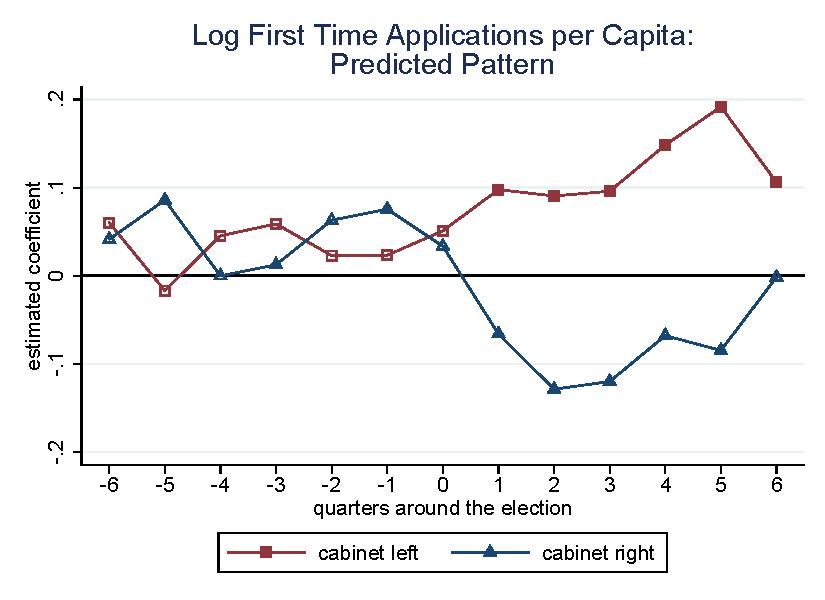
\includegraphics[width=1\textwidth]{app_Graph2.pdf}
    {\footnotesize This figure shows the time evolution of refugee inflows controlling for the type of incumbent cabinet as estimated in the fixed effects regression (1) with a set of dummies for before, during and after the election. Significant coefficients are indicated by filled plot markers. }
	\label{Figure1}
\end{figure}

\begin{figure}
	\centering
    \caption{log First-Time Asylum Applications per Capita: Predicted pattern 6 quarters before and after an election}
	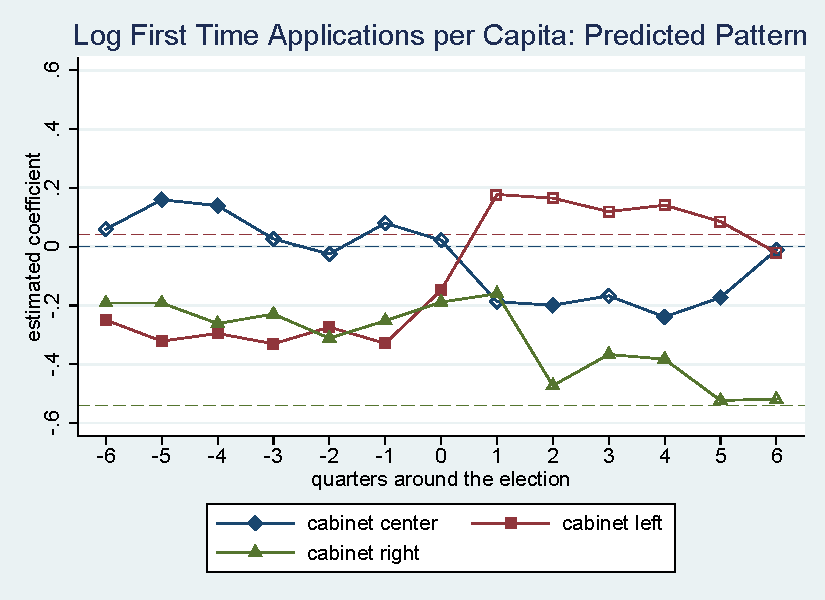
\includegraphics[width=1\textwidth]{app_Graph4.pdf}
	      {\footnotesize This figure shows the time evolution of refugee inflows controlling for the type of incumbent cabinet as estimated in the fixed effects regression (1) with a set of dummies for different quarters before and after an election in a quarter $t=0$. Significant coefficients are indicated by filled plot markers. }\\
\label{Figure2}
\end{figure}

Moreover, we also look at four different asylum decision outcomes: (1) the overall acceptance rate defined as the ratio of all positive decisions to all decisions taken in that quarter, (2) the refugee status rate defined as the ratio of people who were granted full Geneva Convention refugee status to all people seeking refugee status, (3) the temporary protection rate defined as the ratio of other positive decisions to all decisions and (4) the ratio of refugee status decisions to all positive decisions. In order to control for the inflow of asylum seekers, we further include  the log of the yearly total asylum decisions in the destination country as well as the log of  the yearly dyadic asylum decisions in the destination country in our regression equation (1) . The results of the estimation are presented in Table 2.  While our results suggest that overall more asylum applicants are granted some form of protection under left cabinets,  the asylum decision process does not seem to be affected by an election (see Figure 3).  

\begin{figure}
	\centering
    	\caption{Asylum Acceptance Rate: Predicted pattern 6 quarters before and after an election}
	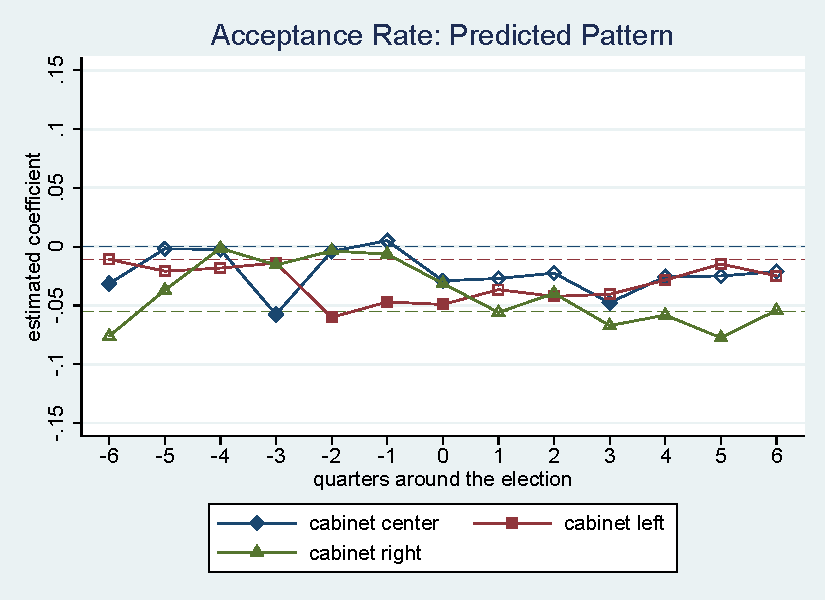
\includegraphics[width=1\textwidth]{acceptance_Graph4.pdf}
       {\footnotesize This figure shows the time evolution of the acceptance rate of asylum applicants controlling for the type of incumbent cabinet as estimated in the fixed effects regression (1) with a set of dummies for different quarters before and after an election in a quarter $t=0$. Significant coefficients are indicated by filled plot markers. }\\
\label{Figure3}
\end{figure}

\begin{table}[htbp]\centering
	\footnotesize
\def\sym#1{\ifmmode^{#1}\else\(^{#1}\)\fi}
\caption{Determinants of asylum decisions}

\begin{tabularx}{\textwidth}{l*{4}{Y}}
\hline\hline
\centering                                        &(1) & (2) & (3) & (4)\\
\centering Dependent Variable &Acceptance  Rate&Temporary Protection Rate & Refugee Status Rate & Refugee in total positive decisions\\
\hline
&\\
Political Terror Scale                  &  -0.00306         &  -0.00621         &   0.00315         &   0.00824         \\
                                        & (0.00995)         & (0.00490)         & (0.00807)         &  (0.0108)         \\
[0.3em]
Civic Liberty (FHI)                     &   0.00577         &   0.00500         &  0.000768         &  -0.00512         \\
                                        & (0.00913)         & (0.00565)         & (0.00752)         &  (0.0238)         \\
[0.3em]
Political Rights (FHI)                  &    0.0128\sym{**} &   0.00243         &    0.0104\sym{*}  &    0.0242         \\
                                        & (0.00447)         & (0.00358)         & (0.00449)         &  (0.0123)         \\
[0.3em]
Battle deaths (000s)                     &   0.00737\sym{***}&   0.00555\sym{***}&   0.00181\sym{***}&  -0.00342\sym{***}\\
                                        &(0.000343)         &(0.000207)         &(0.000392)         &(0.000589)         \\
[0.3em]
log origin country real GDP per capita  &   -0.0488\sym{*}  &   -0.0158         &   -0.0331         &    0.0149         \\
                                        &  (0.0199)         &  (0.0136)         &  (0.0198)         &  (0.0230)         \\
[0.3em]
log destination country real GDP per capita&     0.104         &    0.0194         &    0.0850         &    0.0575         \\
                                        &  (0.0751)         &  (0.0617)         &  (0.0600)         &  (0.0984)         \\
[0.3em]
Unemployment rate at destination        &   0.00261         &   0.00523\sym{*}  &  -0.00262         &  -0.00224         \\
                                        & (0.00242)         & (0.00245)         & (0.00232)         & (0.00515)         \\
[0.3em]
Weighted cabinet position left          &    0.0392\sym{**} &    0.0563\sym{***}&   -0.0171         &    -0.110\sym{***}\\
                                        &  (0.0138)         &  (0.0117)         & (0.00914)         &  (0.0257)         \\
[0.3em]
Weighted cabinet position right         &    0.0196         &    0.0141         &   0.00553         &   0.00919         \\
                                        &  (0.0105)         &  (0.0126)         &  (0.0111)         &  (0.0305)         \\
[0.3em]
yearly total asylum decisions per capita&   -0.0391\sym{***}&   -0.0184\sym{**} &   -0.0207\sym{*}  &   0.00839         \\
                                        &  (0.0109)         & (0.00657)         & (0.00896)         &  (0.0150)         \\
[0.3em]
yearly dyadic asylum decisions per capita&    0.0112         &   0.00562         &   0.00560         &  -0.00104         \\
                                        & (0.00710)         & (0.00333)         & (0.00548)         & (0.00629)         \\
[0.3em]
time period before the election         &  -0.00165         &   0.00721         &  -0.00886         &  -0.00824         \\
                                        & (0.00944)         & (0.00869)         & (0.00682)         &  (0.0202)         \\
[0.3em]
quarter of the election                 &  -0.00620         &   0.00596         &   -0.0122         &   -0.0220         \\
                                        &  (0.0110)         &  (0.0113)         & (0.00746)         &  (0.0236)         \\
[0.3em]
time period after the election          &   -0.0120         &   0.00453         &   -0.0166\sym{*}  &   -0.0685\sym{***}\\
                                        & (0.00640)         & (0.00698)         & (0.00735)         &  (0.0164)         \\
[0.3em]
cabinet position left * before the election&   -0.0407\sym{*}  &   -0.0421\sym{***}&   0.00148         &    0.0632\sym{*}  \\
                                        &  (0.0158)         &  (0.0113)         &  (0.0111)         &  (0.0280)         \\
[0.3em]
cabinet position left * election quarter&   -0.0668\sym{**} &   -0.0635\sym{***}&  -0.00331         &    0.0831         \\
                                        &  (0.0220)         &  (0.0162)         &  (0.0160)         &  (0.0434)         \\
[0.3em]
cabinet position left * after the election&   -0.0242         &   -0.0371\sym{**} &    0.0129         &     0.121\sym{***}\\
                                        &  (0.0150)         &  (0.0112)         &  (0.0103)         &  (0.0236)         \\
[0.3em]
cabinet position right * before the election&   0.00895         &    0.0338\sym{**} &   -0.0248\sym{*}  &   -0.0941\sym{**} \\
                                        &  (0.0131)         &  (0.0111)         &  (0.0117)         &  (0.0275)         \\
[0.3em]
cabinet position right * election quarter&   0.00171         &    0.0361         &   -0.0344         &    -0.109\sym{*}  \\
                                        &  (0.0204)         &  (0.0216)         &  (0.0182)         &  (0.0453)         \\
[0.3em]
cabinet position right * after the election&   -0.0315\sym{**} &   -0.0291\sym{*}  &  -0.00235         &    0.0475         \\
                                        &  (0.0101)         &  (0.0108)         &  (0.0106)         &  (0.0295)         \\
&\\
\hline
Observations                            &     14027         &     14027         &     14027         &      8734         \\
Adjusted \(R^{2}\)                      &     0.098         &     0.056         &     0.055         &     0.031         \\
Mean of Dependent Variable              &     0.260         &     0.130         &     0.130         &     0.523         \\
Fixed Effects                           &     D x O         &     D x O         &     D x O         &     D x O         \\
Destination dummies                     &        No         &        No         &        No         &        No         \\
Quarter-Year dummies                    &       Yes         &       Yes         &       Yes         &       Yes         \\
\hline\hline
\multicolumn{5}{l}{\footnotesize Standard errors in parentheses}\\
\multicolumn{5}{l}{\footnotesize \sym{*} \(p<0.05\), \sym{**} \(p<0.01\), \sym{***} \(p<0.001\)}\\
\end{tabularx}
\end{table}


%Some thoughts about causality:\\
An important question is whether the uncovered patterns can be interpreted as causal effects. On this matter, a few comments are in line. First, the estimation is restricted to elections within the regular electoral calendar. So refugee inflows would not have an impact on the date of the election. In this sense, the estimates identify the causal effect of the electoral period on the admission of refugees. Second, there is a concern that previous refugee inflows would have affected the outcome of the election, biasing the results through an omitted variable problem. Reassuringly, controlling for previous levels of refugee inflow at the country level does not substantially change our results.

Third, there is a question of whether there is reverse causality, in the sense that a party is elected precisely because of the migration policy they intend to apply.\footnote{A recent example is the Green Party in the Netherlands, that refused to take part in a majority coalition because of the stance of other parties on refugee policies \textit{\citep{Economist2017}}.} In this case, the cabinet position is endogenous and the estimates can be understood as an upper bound to the true effect of a given party on the refugee influx.  Unfortunately, the empirical strategy adopted here can do little to address this concern, and other quasi-experimental designs should be explored in the future. Nevertheless, our estimates still show a causal effect of the electoral cycle on the inflow of refugees and uncover an important correlation between the inflow of refugees  and the cabinet's position.

Finally, a deeper question is whether the effects of elections and political parties on refugee inflows are driven by the demand side (the refugees) or the supply side (the incumbent party). Again, as emphasized by the economic literature, asylum seeking behaviors are mainly driven by exogenous factors in the home country. It is difficult to imagine that conditional on the identity of the incumbent party, refugees wait for the outcome of the election to file or not their asylum application. To believe this, one needs to assume that asylum seekers have relatively good knowledge of the political system of the receiving country. Thus, we believe that the effects we capture are mainly driven by the supply side. 

% %%--------------------------------------------------------------------------------------------------
% \section{Introduction}\label{Intro}


% %--------------------------------------------------------------------------------------------------
% \section{Background and determinants of naturalization}\label{Background&Determinants}

% \subsection{Empirical specification}

% \subsection{Data}

% \begin{table}
% \centering
% \caption{Descriptive statistics}
% \small
% \label{tab:sum}
% \begin{threeparttable}
% \begin{tabular}{l rrrrr }

% \end{tabular}
% \begin{tablenotes}[para,flushleft]
% \footnotesize
%  Note: US states between 1986 and 2012.
% \end{tablenotes}
% \end{threeparttable}
% \end{table}



% %--------------------------------------------------------------------------------------------------
% \section{Results}\label{Results}


% \begin{table}
% \centering
% \caption{Basic results}
% \footnotesize
% \label{tab:basic results}
% \begin{threeparttable}
% \begin{tabular}{l*{6}{c}}

% \end{tabular}
% \begin{tablenotes}[para,flushleft]
% \footnotesize
%  Note: Fixed effects estimation including a constant term and a set of state-year characteristics. Robust standard errors clustered by state. t-statistics reported in parentheses and p-values for the AB and Hansen test. Significance levels: {\bf $^{\star\star\star}$} 1\%; {\bf $^{\star\star}$} 5\%; {\bf $^{\star}$} 10\%.
% \end{tablenotes}
% \end{threeparttable}
% \end{table}


% %\begin{figure} 
% %\label{fig:basic} 
% %\centering
%    %\begin{subfigure}[b]{0.8\textwidth}
%    %\includegraphics[width=1\linewidth]{example1.pdf}
%    %\caption{}
%    %\label{fig:dyn1} 
% %\end{subfigure}
% %\begin{subfigure}[b]{0.8\textwidth}
%    %\includegraphics[width=1\linewidth]{example2.pdf}
%   % \caption{}
%    %\label{fig:dyn2}
% %\end{subfigure}
% %\caption[Dynamics during term]{Dynamics during term. Dependent variable: (a) Naturalizations (log). (b) Acceptance rate.}
% %\end{figure}



% \section{Robustness}\label{Robust}


% %--------------------------------------------------------------------------------------------------
% \section{Conclusion}\label{Conclusion}


%--------------------------------------------------------------------------------------------------
% Add Literature

%\small
%\singlespacing

%\onehalfspacing
%\normalsize
%--------------------------------------------------------------------------------------------------
\pagebreak
\bibliographystyle{apalike}
\bibliography{refugee_election}
%\appendix
%%--------------------------------------------------------------------------------------------------
%\section{Additional Figures}\label{app_fig}
%\input{app_figures}
%%--------------------------------------------------------------------------------------------------

\end{document}

